In Figure~\ref{fig:simulation}, a screenshot is shown of the program, while a simulation is running. Note that the shadows are drawn using a generic OpenGL approach, using a particular transformation and drawing the scene twice. This means that the luggage casts a shadow in real-time as well. There are no shadows on other objects (like the luggage belts for example) however, unfortunately. In Figure~\ref{fig:drawing-together} and Figure~\ref{fig:shadow-block} some other aspects of the program are illustrated.

\begin{figure}
  \begin{center}
    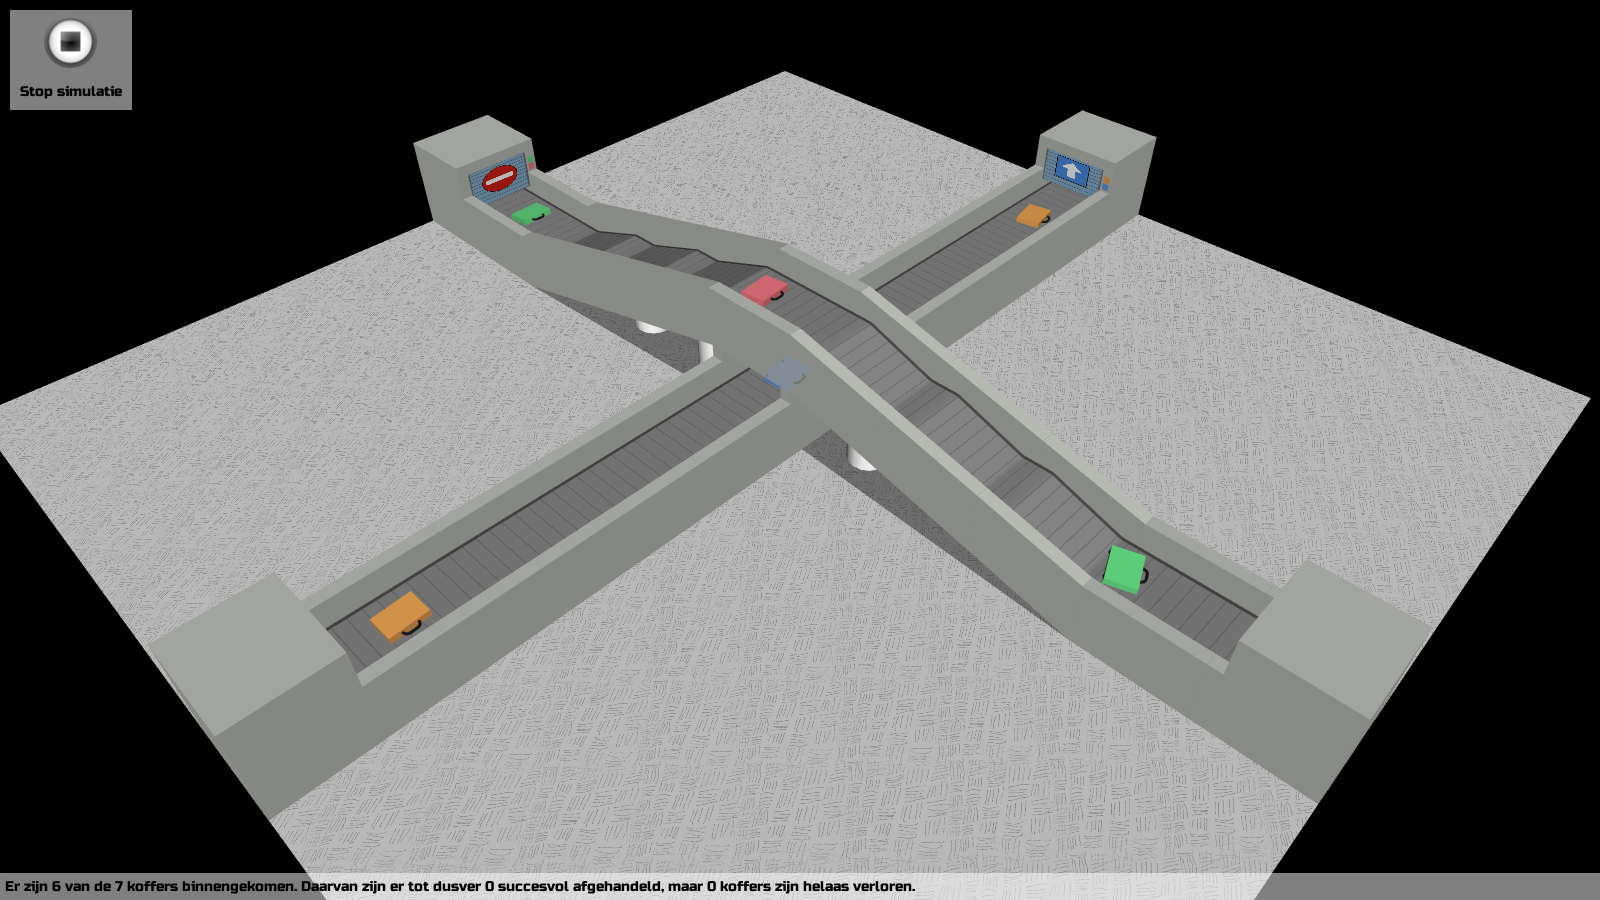
\includegraphics[width=\linewidth]{simulation}
    \caption{Screenshot of the program, showing a running simulation. Note that luggage is always visible, even if it is obscured by other blocks: this can be seen in the center of the image, at the ``bridge''. We did this so that the user will not lose track of luggage.}
    \label{fig:simulation}
  \end{center}
\end{figure}

\begin{figure}
  \begin{center}
    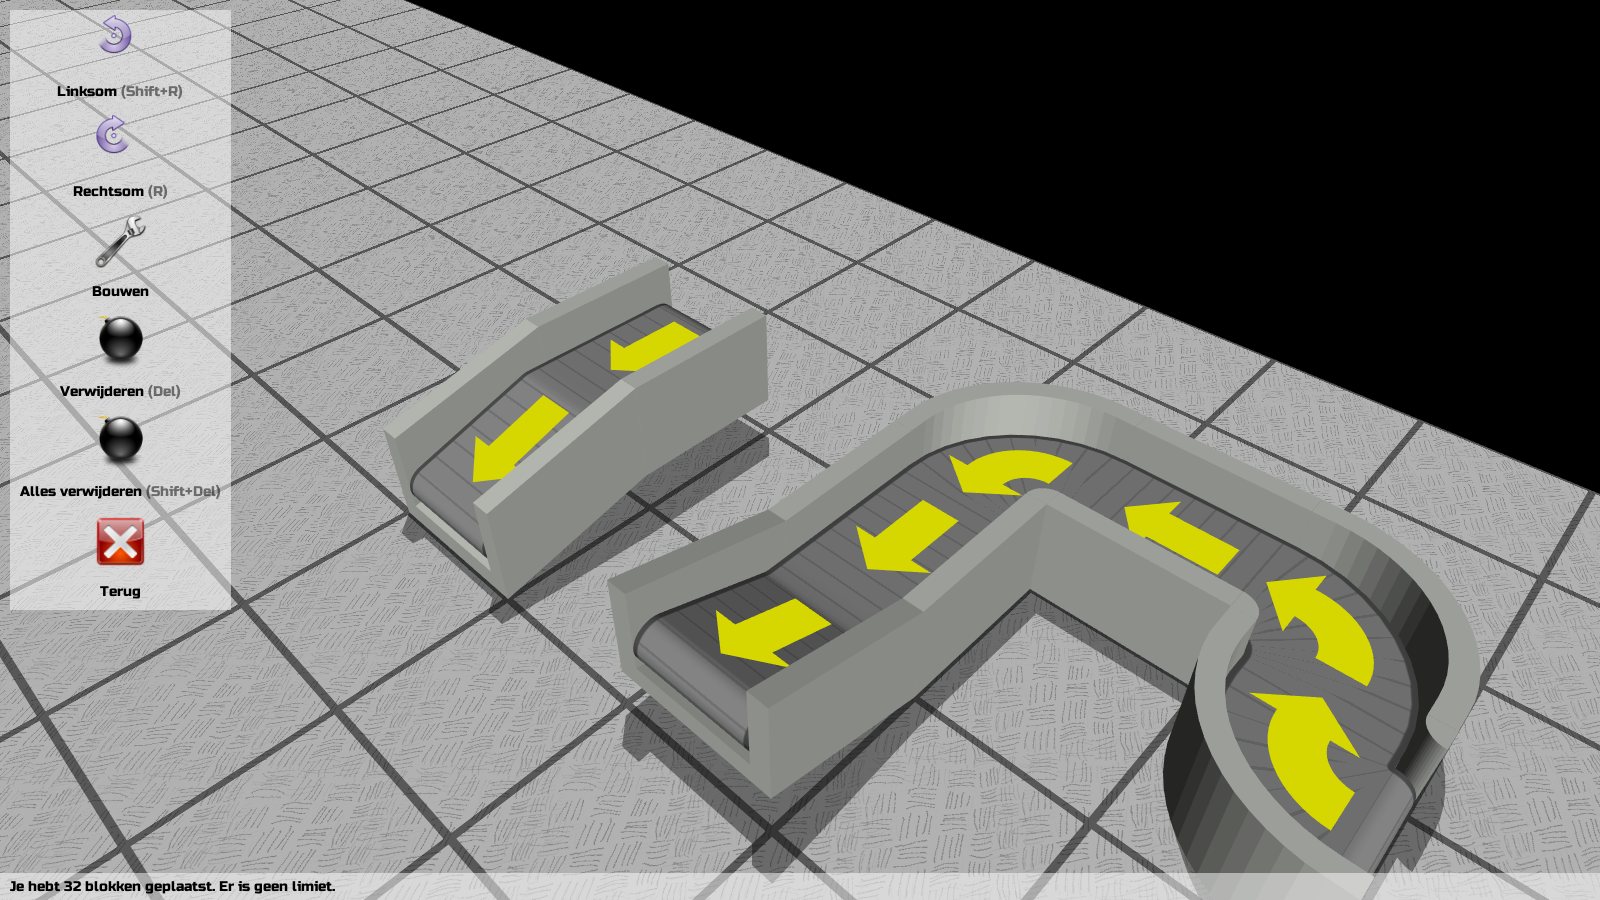
\includegraphics[width=\linewidth]{drawing-together}
    \caption{Adjacent conveyor belts are drawn together as one large conveyor belt.}
    \label{fig:drawing-together}
  \end{center}
\end{figure}

\begin{figure}
  \begin{center}
    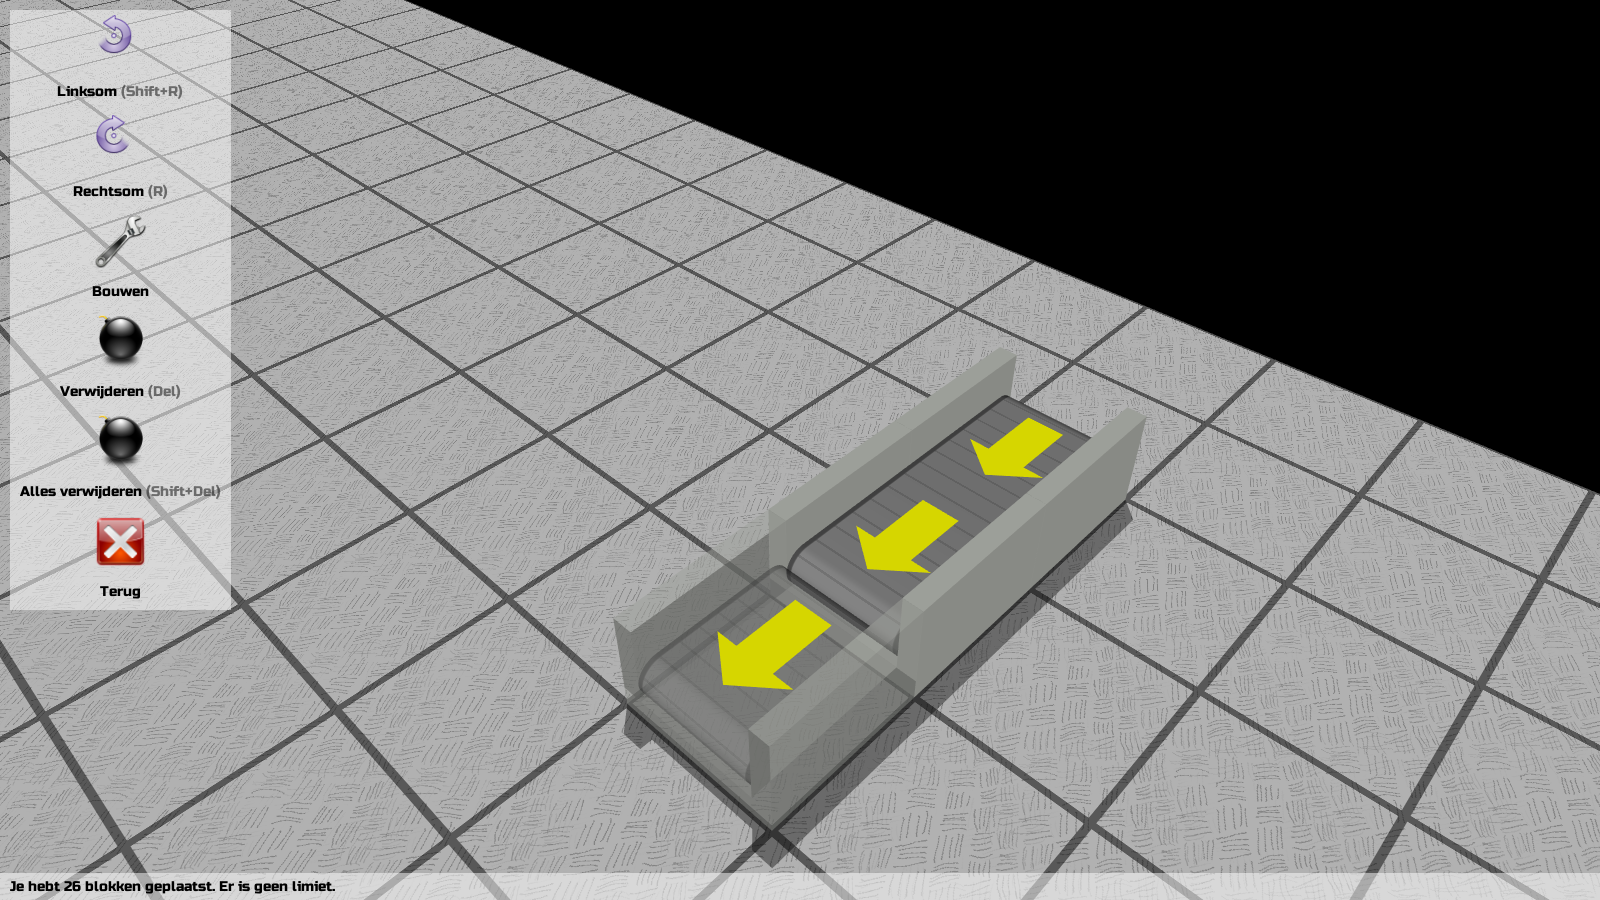
\includegraphics[width=0.45\linewidth]{shadow-block-1}
    \quad
    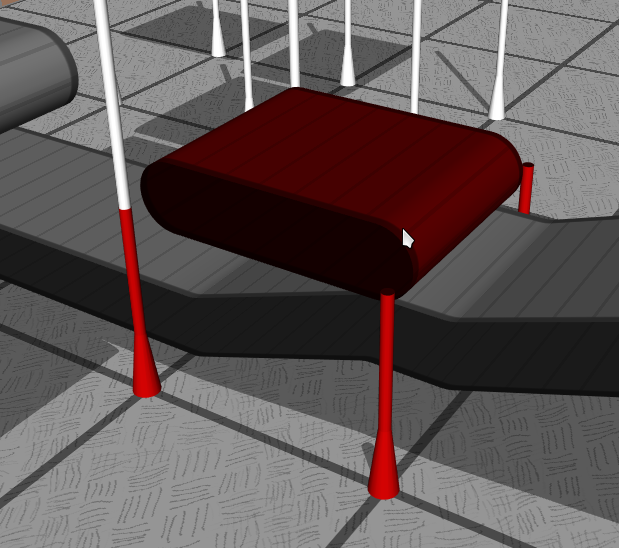
\includegraphics[width=0.45\linewidth]{shadow-block-2}
    \caption{Adding a new block. \textit{Left:} The block that is going to be added is shown as a ``ghost block'' under the cursor. \textit{Right:} If it is not possible to place the block on the indicated location, the ghost block becomes red to show this.}
    \label{fig:shadow-block}
  \end{center}
\end{figure}

% \subsection{To be done}
% There are quite some tasks that still need to be done at the moment.
% \begin{itemize}
%   \item Drawing more details for the conveyor belts (for example the axes are missing at the moment).
%   \item Drawing arrows to show the direction of conveyor belts in the building mode. More general, giving more clues to the user what to do (arrows, et cetera).
%   \item Being able to choose an existing block to start building from (right now, the user needs to indicate the height for every new block by dragging, which is not very efficient).
%   \item Improvements to the graphical interface.
%   \item Adding scanner blocks.
%   \item Making the program more like a game, for example by adding levels and a scoring system.
%   \item Being able to open and save conveyor belt systems.
% \end{itemize}


